\chapter{Review of Literature} \label{review-of-literature}

\section{Architecture} \label{Technology}

\subsection{Introduction} \label{subsec-lr-arc-intro}
\subsection{Summary} \label{subsec-lr-arc-summ}

\section{Technology} \label{Technology}

\subsection{Introduction} \label{subsec-lr-tech-intro}

The aim of this document is to review some of the state-of-the-art technology that can be used to architect the monitoring system for storing and handling big datasets and performing real-time analytics on them. The proposed architecture will consist of three layers: the batch layer, serving layer and speed layer.\\

\subsection{Batch Layer} \label{subsec-lr-batchlayer}

\subsubsection{Introduction} \label{subsubsec-lr-batchlayer-intro}
A batch layer is required to store constantly growing big data and for historical data analysis that is used to identify patterns such as job failures, popular data, busy sites and so forth.  Many individuals consider Hadoop as the de facto framework for analysing big data. However, there are many technologies available in the distributed system such as the Internet that go beyond MapReduce, a programming model for processing big data that was introduced by Google \cite{mr-com} . In this chapter an attempt will be made to review such technologies.\\

\subsubsection{Apache Hadoop- MapReduce and HDFS} \label{subsubsec-lr-batchlayer-mr}
The Hadoop stack has been used for many research and commercial products. It has gone through rigorous implementation and testing, which makes it robust. There are many Hadoop ecosystems and distributions, but in order to make this review relevant to the proposed layer, the MapReduce and Hadoop Distributed File System (HDFS) will be analysed. MapReduce is a programming model that was designed to remove the complexity of processing data that are geographically scattered around the distributed infrastructure \cite{mr-com,mr-data}. It hides the complexity of computing in parallel, load balancing and fault tolerance over a large range of inter-connected machines from developers.\\

There are two simple parallel methods; map and reduce are predefined in the MapReduce programming model and are user-specified methods, so users have control over how the data should be processed \cite{mr-data}. Hadoop was designed taking into account that moving computing to where the data reside is better than vice versa as it will reduce bottlenecks in the network, especially when the data that are being transferred are at the rate of terabytes-to-petabytes \cite{mr-com}. Therefore, map and reduce jobs will be allocated to where the data reside, which will be scheduled by JobTask Manager as shown in Figure \ref{fig-map-reduce}. The data will be read from the local disk (file system); mapped, with all records being independently processed and key/value pairs assigned; intermediate results are stored to the local disk and they are shuffled (transferred to where the reduce jobs are located); and reduced, so that records with identical keys are processed together and the output is written back to the disk (this output could be an input to another MapReduce job) \cite{mr-com}. Fault tolerance in MapReduce is supported by periodically checking the heartbeat of the worker nodes, master failures can be protected against by using check-pointing, an approach used to enable applications to recover from failure.\\

\begin{figure}[H]
\centering
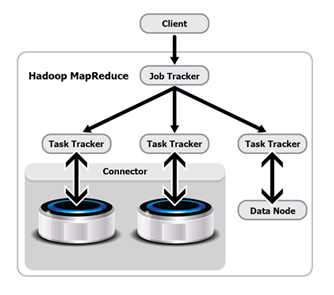
\includegraphics[width=0.5\textwidth]{Figures/map-reduce.png}
\caption{Hadoop Architecture}\label{fig-map-reduce}
\end{figure}

The MapReduce framework is built on HDFS and executes I/O operations on it. The HDFS guarantees: scalability on commodity hardware, fault tolerance, high throughput, load balance, data integrity and portability \cite{intro-hdfs}. It employs master-slave architecture, which is prone to single point failure. However, it facilitates failover to the standby server but this is prone to downtime. Data are replicated across disk nodes for load balancing, fault tolerance and high availability \cite{intro-hdfs}.

\subsubsection{Stratosphere} \label{subsubsec-lr-batchlayer-stratosphere}
Stratosphere extends the MapReduce model as discussed in section \ref{subsubsec-lr-batchlayer-mr} with new operators such as union, iterate, join, cross and cogroup as shown in Fig. 2. All operators will start working in the memory and when there isn’t enough memory then the rest of the data will be processed from the disk. The principal concept in Stratosphere is Parallelisation contracts (PACTs), which categorises three types: input contract, which suggests how inputs to compute nodes are structured; user function, which enables developers to program how to transform from inputs to outputs and output contract, which offers compiler hints to achieve performance improvement (4). PACTs are data processing objects in the data flow. Input data go through nodes for transformation, computation, and optimisation in parallel. Stratosphere distributes the resource manager and execution engine called Nephele, which utilises a master-slaves structure where the single master node receives a job graph from the upper layer as grounds to apply for resources by communicating with the resource administrative unit that is used to manage the computing resources of slave nodes (4). When adequate resources are available for a certain job, the master node distributes tasks to slave nodes and keeps track of their progress such as initialisation, running, completion and so forth.

\begin{figure}[H]
\centering
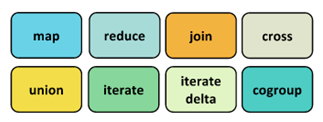
\includegraphics[width=0.5\textwidth]{Figures/stratosphere.png}
\caption{Stratosphere Operators}\label{fig-stratosphere}
\end{figure}

\subsubsection{Apache Spark} \label{subsubsec-lr-batchlayer-spark}
Apache Spark is an in-memory distributed computing framework (5, 6). It provides a general programming model supporting iterative classes of algorithms, interactive applications and algorithms containing common operators such as Map, Reduce, Join, Filter, GroupBy, Sort, LeftOuterJoin, RightOuterJoin, Count, Union, Cross and so forth (5). Spark allows the dataset to be kept in the memory by moulding a new memory abstraction, called Resilient Distributed Datasets (RDDs) (6). Instead of repeated I/O operation, Spark fetches the dataset once from the file system and directly accesses it from the memory thereafter, which improves the performance. By storing intermediate results in the memory, it provides a mechanism for reusing the data to perform other operations such as iteration. 

\subsubsection{Comparison} \label{subsubsec-lr-batchlayer-comparison}
MapReduce is largely believed to be a solution for batch processing (1). However, MapReduce barely deals with the instances where the development of procedures requires the arbitrary mixture of a set of operations, iterative jobs and multiple inputs. Nevertheless, the above mentioned actions could be achieved by implementing multiple map and reduce operations. On the contrary, reloading the same data multiple times from the disk will seriously downgrade the performance. The Spark and Stratosphere provided a mechanism for overcoming this issue by using inbuilt in-memory processing and extending the MapReduce framework to support many operators such as: join, group, iterate, union and cross as shown in Table. 1.

\begin{figure}[H]
\centering
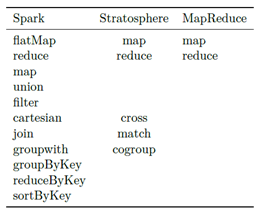
\includegraphics[width=0.5\textwidth]{Figures/batch_comparison.png}
\caption{Operators comparison}\label{fig-batch-comparison}
\end{figure}

In brief, MapReduce, Stratosphere and Spark have some common features: load balancing, and fault tolerance. Stratosphere extends MapReduce, offering further operations as shown in Fig. 2. Spark provides the in-memory processing mechanism and supports the interactive analyses. On the other hand Stratosphere offers optimisation mechanisms.

\subsection{Serving Layer} \label{subsec-lr-servinglayer}

\subsubsection{Introduction} \label{subsubsec-lr-servinglayer-intro}
Batch processing jobs are expected to run for hours, weeks, months or even years, which is not ideal for monitoring a data- infrastructure such as WLCG. Therefore, a serving layer is required for ad-hoc interactive queries. A few well known intensive Internet giants have developed tools to resolve this issue, which will be reviewed in the following section.

\subsubsection{Apache Drill} \label{subsubsec-lr-servinglayer-drill}
Apache Drill is a distributed execution engine that facilitates interactive, ad-hoc querying heterogeneous data sources on a large scale, which was inspired by Google's Dremel (7, 8). Its design goal is to scale to 10,000 servers or more and to process petabytes of data and trillions of records in seconds (8). As shown in Fig. 4, Drill’s architecture is made up of four components: query languages, which is responsible for parsing the user’s query and constructing an execution plan; a low-latency distributed execution engine that provides the scalability and fault tolerance needed to efficiently query petabytes of data; nested data formats, which are responsible for supporting various data formats (8). The initial goal is to support the column-based format used by Dremel (8). Finally, scalable data sources are responsible for supporting a variety of data sources. The initial focus is to leverage Hadoop as a data source (8).

\begin{figure}[H]
\centering
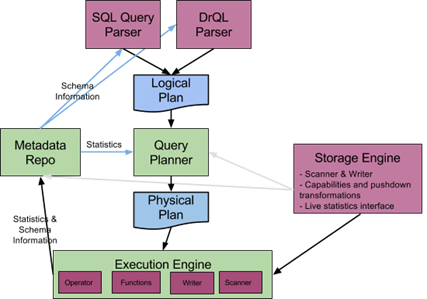
\includegraphics[width=0.5\textwidth]{Figures/drill.png}
\caption{Apache Drill Architecture}\label{fig-serving-drill}
\end{figure}

From a distribution perspective, Drillbits, each node’s instance of Drill, uses local memory and data. Queries can be made from any such instance (8). The co-ordination, query planning and optimisation, scheduling, and execution are then distributed.

\subsubsection{Cloudera Impala} \label{subsubsec-lr-servinglayer-impala}
Cloudera Impala is a massively parallel processing (MPP) architecture for performing SQL-like queries on HDFS and HBase storage as shown in Fig. 4, which does not employ the MapReduce model as other alternatives such as Hive (9). It leverages techniques such as columnar storage for performing really fast scans in the order of seconds of huge amounts of data in memory. All data in HDFS or HBase do not require Extraction, Transformation and Loading (ETL) so can be queried directly without any data movement or predefined schemas using SQL-like commands. Impala inherits inbuilt Hadoop security by integrating with Kerberos for authentication and role-based authorisation (9).

\begin{figure}[H]
\centering
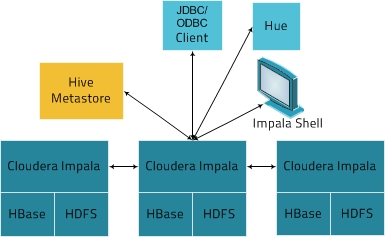
\includegraphics[width=0.5\textwidth]{Figures/impala.png}
\caption{Cloudera Impala}\label{fig-serving-impala}
\end{figure}

\subsubsection{Facebook’s Presto} \label{subsubsec-lr-servinglayer-presto}
Presto is a distributed low-latency, interactive and SQL-compliant query engine optimised for ad-hoc analysis (10). It also supports the majority of ANSI SQL subgroups, including complex queries, aggregations, joins, and window functions (10). All processing is carried out in-memory and pipelined across the network between steps, which should reduce the read/write to disk thus improving performance. The shortcomings of the system are its inability to write output data back to tables as it only supports the read-only mode. In Presto architecture as shown in Fig. 5, there is a coordinator that receives SQL queries from the client, which it then analyses, parses and then plans the execution (10). Then the scheduler connects the execution pipeline and assigns the jobs to worker nodes that reside closer to the data (10). The client then fetches the results.

\begin{figure}[H]
\centering
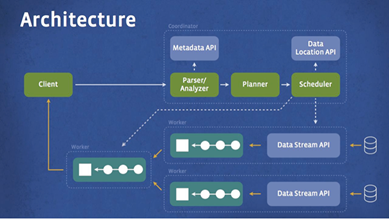
\includegraphics[width=0.5\textwidth]{Figures/presto.png}
\caption{Presto Architecture}\label{fig-serving-presto}
\end{figure}

The Presto framework is extendable so any storage can be plugged in; however, it require a connector that provides Presto with metadata, information on which nodes hold the data, and a way to actually fetch the data as a stream. The current version provides plugins for the following storage system: HDFS, Hive, HBase and Scribe (10).

\subsubsection{Apache Shark} \label{subsubsec-lr-servinglayer-shark}
Shark is a large-scale distributed and fault-tolerant, in-memory analytics system designed to be compatible with Hadoop (11, 12). In particular, Shark is fully compatible with Hive and supports HiveQL, Hive data formats, user-defined functions, HDFS, HBase and Amazon S3 (11). Shark provides the users with a mechanism to store or load their working set of data into custom columnar in-memory store and compresses them in order to reduce the storage space and execution time. Shark is a component that sits on top of Spark as shown in Fig. 6, which was discussed in the previous section. It also supports advanced techniques such as data co-partitioning and incorporation of machine learning into the workflow (12). Shark architecture contains an optimiser engine called partial DAG execution, which uses historical data information to dynamically adjust query and execution plans (12).

\begin{figure}[H]
\centering
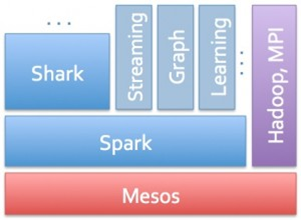
\includegraphics[width=0.5\textwidth]{Figures/shark.png}
\caption{Spark stack}\label{fig-serving-shark}
\end{figure}

\subsubsection{Comparison} \label{subsubsec-lr-servinglayer-comparison}
Hadoop was never built for real-time interactive ad-hoc querying; it mainly focuses on offline batch processing. This has resulted in a need for a new stack of technologies that could resolve high latencies. In recent years a few tools have emerged to address this issue, which have been listed in a previous section. In brief, Drill, Impala, Presto and Shark were developed to take advantage of in-memory temporary data locality. Spark and Drill support long-running queries and ad-hoc queries, whereas Impala and Presto do not support long running queries.

No fault-tolerance is implemented in Impala or Presto; when a node fails at the execution time then the queries need to be re-executed. However, Shark utilises an underlying Spark engine for fault-tolerance by exercising the lineage method, which is a technique used to recover missing pieces of RDDs by re-computing or rebuilding from the row data source (12). Impala and Shark were designed to take advantage of the existing Hive infrastructure, which uses the same metadata. In contrast, Drill and Presto were developed to provide distributed query abilities across various data stores. However, the current framework only supports Hadoop. Some of the published benchmarks state that Shark performs much better than Impala and Presto (13). However, there aren’t any benchmarks to compare it with Drill due to the fact that it is still under development. Shark provides a mechanism to utilise complex machine learning to embed with the analytics dataflow; however, Drill, Presto and Impala do not support this.

\subsection{Real-Time Layer} \label{subsec-lr-servinglayer}

\subsubsection{Introduction} \label{subsubsec-lr-reallayer-intro}
A speed layer is required to perform real-time analytics on fresh data as they are received. This is required to monitor the infrastructure proactively and trigger actions so the operation will run smoothly.

\subsubsection{Apache Storm} \label{subsubsec-lr-reallayer-storm}
Apache Storm is a distributed, real-time processing of unbounded streams of the data system (14). It is considered as an alternative to high-latency batch processing for processing data in low-latency near real-time. Storm can be embedded with the queuing and database technologies. It facilitates scalability by enabling users to determine how many worker nodes are required to execute a job and the number of parallelism (threads) on the topology configuration. It also uses an independent Apache technology called Zookeeper for coordinating the cluster, which also supports a cluster scale (14). The architecture employs a master-slave model (14). The master node has a daemon called Nimbus, which is responsible for distributing user applications to worker nodes, allocating jobs to the worker queue and monitoring the status of the worker nodes, which on failure will restart the node or reassign the task to other nodes (14). The slave nodes have a daemon called supervisor, which is accountable for checking the queue for new jobs (14). 

\begin{figure}[H]
\centering
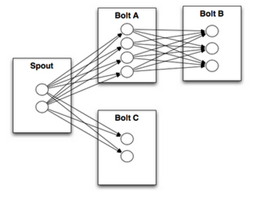
\includegraphics[width=0.5\textwidth]{Figures/storm.png}
\caption{Storm topology}\label{fig-real-storm}
\end{figure}

Storm uses tuples as its data model, which consists of a list of values. Groups of spouts and bolts are packaged into a topology, which is then deployed into clusters that will run infinitely, until killed manually. As shown in Fig. 7, the topology will consist of spouts, which are the source of streams; bolts, which consume the stream and process them; and stream grouping, which states how the data should flow (14). Storm also provides a tool called Distributed RPC, which enables developers to implement complex functions and execute them in Storm utilising parallelism.

\subsubsection{Simple Scalable Streaming System (S4)} \label{subsubsec-lr-reallayer-s4}
S4 is a distributed general-purpose platform that processes continuous unbounded streams of data (15). S4 employs the MapReduce and Actor programming models (15). Therefore, S4 utilises concurrent, decentralised and symmetric architecture, with each node sharing the same functionality and responsibility, which is imposed by utilising Apache ZooKeeper in order to coordinate the cluster. There aren’t any special nodes with special functions. The S4 model facilitates high availability and scalability on commodity hardware, low-latency by utilising local memory, fault-tolerance by check-pointing and summoning the standby server to take over the failed server tasks, and a pluggable framework so that it's more generic and new components can be plugged in (15).

\begin{figure}[H]
\centering
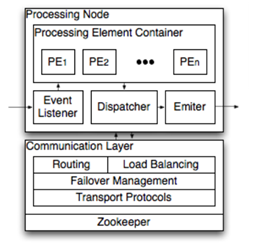
\includegraphics[width=0.5\textwidth]{Figures/s4.png}
\caption{S4 Architecture}\label{fig-real-s4}
\end{figure}

As shown in Fig. 8 processing nodes are the logical clusters of Processing Elements (PE), an entity that performs computation and transmits messages between PEs by using data events. The processing nodes are responsible for listening to events, executing functions on the incoming events, transmitting events and emitting output events. An event listener in the PN passes incoming events to the processing element container, which invokes the correct PEs corresponding to the unique key or generates a new instances of PEs (15). An application can be defined in terms of PEs with simple processing logic, and the framework instantiates one PE for each unique key in the stream. The communication layer provides load balancing, failover management and transport management (15). There are numerous special PEs that are available for performing tasks such as: count, aggregate, join and so forth (15).

\subsubsection{Amazon Kinesis} \label{subsubsec-lr-reallayer-kinesis}
Amazon Kinesis is a cloud-based service for real-time processing of high-volume stream data (16). Just as with any cloud service the Kinesis service is based on a metering system, which means you pay for the amount of throughputs and HTTP PUTs transactions used (16). Kinesis is proficient at consuming any amount of data from any number of sources, scaling up and down as needed. The Kinesis client library supervises load balancing, coordination and error handling automatically, so the developer only needs to focus on processing the data as it becomes available.

\begin{figure}[H]
\centering
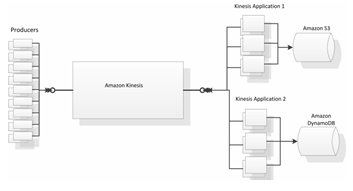
\includegraphics[width=0.5\textwidth]{Figures/kinesis.png}
\caption{Kinesis Architecture}\label{fig-real-kinesis}
\end{figure}

As shown in Fig. 9, Kinesis expects two components, which are the producer and worker (16). The producer accepts data from a source and converts them into a Kinesis stream, which is partitioned into 50KB data segments, then transferred into stream using HTTP PUTs methods (16). The worker then takes the data from the Kinesis stream and processes them. For scalability, the user has to take care of two things; adding or removing shards, depending on the required throughput capacity, and using the Kinesis client library and deploying the application into EC2 instance with the auto-scaling group.

\subsubsection{Apache Samza} \label{subsubsec-lr-reallayer-samza}
This is a distributed stream processing pluggable framework to run continuous computation on infinite streams of data (17). It’s designed to sit on top of the Kafka messaging queue for stream processing. It also utilises Apache Yet Another Resource Negotiator (YARN) for resource management and execution, which is responsible for deploying tasks in a distributed clusters, stream processor locality, co-partitioning of streams and providing security (17). The Samza framework is similar to batch processing as shown in Fig. 10.

\begin{figure}[H]
\centering
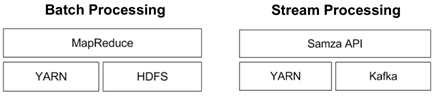
\includegraphics[width=0.5\textwidth]{Figures/samza.png}
\caption{Samza Architecture}\label{fig-real-samza}
\end{figure}

Samza partitions the message, assigns the partition key and sequence ID, and orders them in strict sequence. All messages matching the partition key would go to that partition.

It also facilitates a replayable mechanism so that a message can be reread when required. The stream processing is done by Samaza Job, which performs logical transformation on a set of input and emits outputs (17). Fault tolerances are managed by check-pointing, which enables failure recovery, and state management. This maintains the state of the intermediate data that need to be passed between processing; this is kept in the local disk with each task (17).

\subsubsection{Spark Streaming} \label{subsubsec-lr-reallayer-spark}
Spark Streaming is an extension of Spark that supports continuous processing (18, 19). As shown in Fig. 11, Spark Streaming is inspired by a batch system, such as dividing processing into sufficient sets so  that they can be replayed, assigning failed tasks to other nodes and decreasing batch sizes to tackle low latency (18).

\begin{figure}[H]
\centering
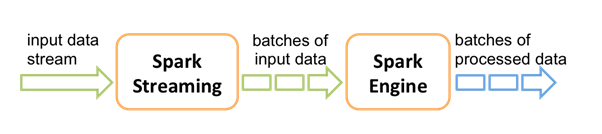
\includegraphics[width=0.5\textwidth]{Figures/spark_stream.png}
\caption{Spark Streaming data flow}\label{fig-real-spark}
\end{figure}
Spark Streaming provides two types of operators for building stream applications: transformation operators, which produce a new DStream from one or more parent streams, and output operators, which let the program write data to external systems (18). Spark Streaming supports all operators that are supported in Spark such as: Map, Reduce, GroupBy, Join and so forth. It also provides a mechanism to aggregate within a given window of time. It also allows the developer to apply Spark’s in-built machine learning algorithms, and graph processing algorithms on data streams (19). It supports checking pointing and fault tolerance, which it inherits from Spark.

\subsubsection{Comparison} \label{subsubsec-lr-reallayer-comparison}
The existing large-scale MapReduce data-processing platforms are highly optimised for batch processing, which typically operates on static data. Therefore, a paradigm was required to process data in real-time so business critical decisions can be made on time. This is where the evolution of the stream processing technologies listed above evolved.  

Storm, S4, Samza, Spark Streaming and Amazon Kinesis share the same aim, which is to provide a distributed, scalable and fault-tolerance infrastructure for processing continuous streams of data. Storm, Kineses, Samza and S4 are fundamentally like a pipeline where the source pushes discrete messages, which are then processed a record at a time. On the other hand, Spark Streaming follows a batch processing model where messages are collected and then processed at short-time intervals in a batch manner. However, this is prone to seconds-latencies compared with former technologies. Nevertheless, Spark does not replicate messages or checkpoints as a mechanism for fault-tolerance as with the other systems, which are liable to high disk I/O, network bandwidth usage and overheads of the operations itself. Spark utilises in-memory storage abstraction (RDD), which tracks the lineage steps used to build it, so in the event of failures, it can recompute the lost data using the cached steps. Storm does not support managing states, whereas S4, SAMZA and Kinesis provide tools to manage them locally or remotely. Storm is user-oriented, as it gives full control to the developers on how it should be configured so an external database can be used to store the states; however, this is costly, in terms of performance. Nevertheless, Samza provides a much better mechanism to minimise remote communication by keeping the state located locally with the tasks and only when a state is modified, will it invoke a remote method for an update. To the best of knowledge all the stream platforms discussed above utilise an in-memory mechanism for processing, except for Amazon Kinesis. Although in-memory processing accelerates low-latencies, this could raise a new issue in terms of flushing out the memory, in particular for S4. A complex application in utilising the S4 framework will generate a large number of unique processing elements as it has been designed to do so, which will occupy a large portion of the memory and could degrade performance. However, there is a mechanism called Time-to-Live that explicitly configures how long the PE should live without any event communication before the memory is reclaimed, but this will result in loss of the state of the PE. However, there is a method to overcome this issue by applying priority or importance of the PE object, which will be customised to the developer.

\subsection{Summary} \label{subsec-lr-tech-summ}
In the previous section, a brief overview of the different technology that supports batch processing, interactive ad-hoc queries and real-time analytics is reviewed. Most of the technology was developed by companies concentrating on their use cases. For some, performance is important, whereas for others fault-tolerance and recovery are important, and only one can be achieved by trading-off the other. So it’s not practical to have a perfect technology tailored for one requirement. Therefore, it’s important to distinguish and prioritise what is essential for the desired system and what can be compromised. 

When you have separate technologies for each layer such as batch/ serving / speed layers, it will become very difficult and complex to maintain the infrastructure. Hence, it will be interesting to explore the Spark stack as it supports batch processing, ad-hoc querying and stream processing. It uses the same processing model and data structures for batch processing and Spark Streaming, which enables ad-hoc queries on streams and combines streams with historical data using the same high-level APIs. Therefore, it simplifies development, deployment and maintenance as the codes can be reused between layers.

